\section{Practical thresholds via a permutation approach}\label{section::permutation}

% Recall that the threshold via Rademacher complexity overestimates the quantile function of the observed distance for each $\theta \in (0,1)$ under the null hypothesis. Even though, for a fixed probability level $\theta,$ we can obtain a rejection region with probability $1 - \theta,$ as long as $n$ and $m$ are sufficiently large, that region is much smaller than the region corresponding to the true quantile. The remedy for this is to use the permutation approach. 

In this section, we introduce a permutation-based framework for two-sample testing that yields improved performance in practice. As discussed earlier, the threshold derived from Rademacher complexity is overly conservative, resulting in low power for finite sample sizes. The permutation approach alleviates this issue by providing a more accurate approximation of the quantile function of the test statistic under the null hypothesis $H_0,$ while typically yielding a much smaller threshold under the alternative.
% In this section, we introduce a more practical approach for two-sample testing via the permutation approach. Recall, that the main problem of the threshold obtained via Rademacher complexity was that it was very large for practical applications. Threshold via permutation approach remedies that problem. In particular, it provides a better approximation for the quantile function of the observed random variable under $H_0$, and whenever null hypothesis is false, it does not require as large an amount of data to make a rejection. The intuition behind this is that the threshold via permutation depends on the laws of random probabilities that generated the data, whereas the threshold via Rademacher complexity works uniformly over all laws of RPM's. Let us now introduce the permutation approach.
% This is done by first obtaining approximate samples of the observed distance and then computing the empirical quantile. The practical advantage of this approach is that, since the quantile is estimated from approximate samples of the test statistic, the rejection region is larger than that obtained via the threshold based on Rademacher complexity. This is intuitive, since the latter works uniformly over all laws of random probability measures, while the former is derived from the data-generating laws $Q^1$ and $Q^2.$ 
Recall that, given $Q^1,Q^2\in \probprobx$, we observe
\[
\widehat{P}^1_{1,m},\cdots, \widehat{P}^1_{n,m} \overset{\iid}{\sim} Q^{1,(m)}, \quad 
\widehat{P}^2_{1,m},\cdots, \widehat{P}^2_{n,m} \overset{\iid}{\sim} Q^{2,(m)}.
\]
Using these samples, we compute the distance $d(\widehat{Q}^1_{n,m}, \widehat{Q}^2_{n,m})$, where $d$ can be either WoW or HIPM. Our goal is to estimate the quantile function of the random variable $d(\widehat{Q}^1_{n,m}, \widehat{Q}^2_{n,m})$ assuming that $Q^1 = Q^2,$ and use it as a testing threshold. Ideally, such a quantile could be estimated empirically from multiple independent realizations of this random variable. In practice, however, only a single realization is available.

We circumvent this limitation by noting that under the null hypothesis $Q^1 = Q^2$, all random probability measures $\widehat{P}^k_{i,m}$ share the same distribution. Consequently, if we randomly shuffle these objects and recompute the distance, the resulting value constitutes another realization from the distribution of $d(\widehat{Q}^1_{n,m}, \widehat{Q}^2_{n,m})$. By repeating this process, we can obtain several samples of the distance between hierarchical estimators. Although these samples are not independent, this dependence is typically negligible in practice when the sample sizes $n$ and $m$ are sufficiently large.

We now formalize this procedure. Recall the hierarchical estimators 
\[
\widehat{Q}^1_{n,m} = \frac{1}{n} \sum_{i = 1}^n \delta_{\widehat{P}^1_{i,m}} \quad \text{and} \quad \widehat{Q}^2_{n,m} = \frac{1}{n} \sum_{i = 1}^n \delta_{\widehat{P}^2_{i,m}}.
\]
To implement the permutation test, we first form the pooled collection of random probability measures
\[
\left\{ \widehat{P}_{1,m},\cdots, \widehat{P}_{2n,m}  \right\} :=\left\{ \widehat{P}^1_{1,m}, \dots, \widehat{P}^1_{n,m}, \widehat{P}^2_{1,m}, \dots, \widehat{P}^2_{n,m} \right\} .
\]
A random permutation of this collection is induced by a vector $R = (R_1, \dots, R_{2n})$ sampled uniformly from the set of all permutations of $\{1, \dots, 2n\}$. For notational brevity, we omit the explicit dependence of $R$ on $n$ and $m$.

We then define the permuted hierarchical estimators as
\[
\widetilde{Q}^1_{n,m} = \frac{1}{n} \sum_{i = 1}^n \delta_{\widehat{P}_{R_i,m}} \quad \text{and} \quad \widetilde{Q}^2_{n,m} = \frac{1}{n} \sum_{i = n+1}^{2n} \delta_{\widehat{P}_{R_i,m}}.
\]
Finally, we compute the distance $d(\widetilde{Q}^1_{n,m}, \widetilde{Q}^2_{n,m}).$

Repeating this process, randomly permuting the pooled sample and recomputing the distance, yields the approximate samples of the distance between the hierarchical estimators of $Q^1$ and $Q^2$. Then, for a given significance level $\theta \in (0,1),$ we set the testing threshold equal to the empirical $(1-\theta)$-quantile of these values.

In practice, since we work with the hierarchical samples $\mathbf{X}_{n,m}, \mathbf{Y}_{n,m}$ permutation is implemented by exchanging the rows between or across them. The resulting procedure is summarized in Algorithm~\ref{algorithm::permutation_approach}.

\begin{center}
\begin{minipage}{0.85\textwidth} % Adjust 0.85 to make it narrower or wider
\begin{algorithm}[H]
\caption{Permutation test with $d \in \{\dlip,\WW\}$}
\label{algorithm::permutation_approach}
\begin{algorithmic}[1]
\Require Hierarchical samples $\mathbf{X}_{n,m},\mathbf{Y}_{n,m}$; significance level $\theta \in (0,1)$; number of permutations $n_\text{perm}$
\Ensure Decision: $1$ = reject $H_0$, $0$ = do not reject $H_0$

\State $T_{\mathrm{obs}} \gets d(\mathbf{X}_{n,m},\mathbf{Y}_{n,m})$ \Comment{Observed test statistic}
\State $\mathcal{Z} \gets \text{vcat}(\mathbf{X}_{n,m},\mathbf{Y}_{n,m})$ \Comment{Pool the $2n$ rows}
\For{$i=1,\ldots,n_\text{perm}$}
    \State $R \gets \text{permute}(\{1,\ldots,2n\})$
    \State $T_i \gets d(\mathcal{Z}_{R_{1:n}}, \mathcal{Z}_{R_{n+1:2n}})$ 
\EndFor

\State $r_\theta \gets \widehat{q}_{1-\theta}(T_1,\ldots,T_{n_\text{perm}})$ \Comment{Empirical $(1-\theta)$-quantile}
\State \Return $\mathbf{1}\{T_{\mathrm{obs}} > r_\theta\}$
\end{algorithmic}
\end{algorithm}
\end{minipage}
\end{center}

The theoretical properties of the proposed procedure are studied by analyzing the asymptotic distributions of the observed test statistic and the corresponding threshold under the null and alternative hypotheses. To this end, we appropriately rescale the observed distance and define the test statistic
\[
T_{n,m} = \sqrt{\frac{n}{2}}\dlip\left( \widehat{Q}^1_{n,m}, \widehat{Q}^2_{n,m} \right).
\]
The corresponding threshold is defined as
\[
r(n,m,\theta) = \inf \left\{ t \in \R : \mathbb{P}\left(\widetilde{T}_{n,m} > t \right) \leq \theta \right\},
\]
where 
\[
\widetilde{T}_{n,m} = \sqrt{\frac{n}{2}} \, d(\widetilde{Q}^1_{n,m}, \widetilde{Q}^2_{n,m}).
\]
Note that this scaling is introduced solely for theoretical analysis and is not required for the practical implementation of the algorithm.

In this section, we restrict attention to the case $d=\dlip$. Deriving the asymptotic distribution of $T_{n,m}$ depends on whether the function class over which the corresponding integral probability metric is defined is a Donsker class (see the proof of Theorem~\ref{theorem::asympt_distr_dlip}). At present, we are unable to verify this property for the WoW distance, and therefore do not establish the theoretical guarantees.

To conclude, we establish asymptotic level-$\theta$ control and consistency guarantees for the proposed testing scheme.
\begin{theorem}[Consistency of permutation approach]
\label{theorem::perm__consistency_dlip}
Given $\X = [a,b]$, and $Q^1, Q^2 \in \probprobx$. Let $\theta$ denote the significance level and $r(n,m, \theta)$ be a threshold from permutation approach. Then
\begin{itemize}
    \item if $Q^1 = Q^2,$ then $$ \limsup_{n,m\to \infty} \mathbb{P}\left(T_{n,m}>r(n,m, \theta)\right)\leq \theta.$$
    \item if $Q^1 \neq Q^2,$ then $$ \lim_{n,m\to \infty} \mathbb{P}\left(T_{n,m} > r(n,m,\theta) \right) = 1.$$
\end{itemize}
\end{theorem}
% Let us see how the threshold via the permutation approach works in practice. We are interested in the type I error, (false positive rate, FPR), and true positive rate (TPR) of the testing scheme, meaning:
% \begin{itemize}
%     \item Given two hierarchical samples from the same laws of RPM, how often does the testing scheme reject the null hypothesis?
%     \item Given two hierarchical samples from two different laws of RPM, how often does the testing scheme reject the null hypothesis?
% \end{itemize}
% In addition to Type I error and TPR, we look at the trade-off between them, i.e., we plot the ROC curve that shows the behaviour of TPR as a function of the FPR.
% In the first figure we are working with the random probability measure defined as
% \begin{align*}
% &\widetilde{P}^1  = \text{TN}(\mu_1, 1) \quad \text{where }\mu_1\sim \mathcal{N}(1.0, 1)\\
% &\widetilde{P}^2  = \text{TN}(\mu_2, 1) \quad \text{where }\mu_2\sim \mathcal{N}(1.5, 1),
% \end{align*}
% where TN denotes the truncated normal distribution on [0,1]. We set the number of permutations equal to $80.$ To get the false positive and true positive rates, we simulate hierarchical measures from the pairs $\left(\mathcal{L}\left(\widetilde{P}^1 \right),\mathcal{L}\left(\widetilde{P}^1 \right) \right)$ and $\left(\mathcal{L}\left(\widetilde{P}^1 \right),\mathcal{L}\left(\widetilde{P}^2 \right) \right).$ We study the two cases: On the first row of Figure~\ref{fig:normal_normal}, $n = 35, m = 10$, and on the second row $n = 70, m = 15.$

% \begin{figure}[h!]
%     \centering
%     \begin{subfigure}{0.32\textwidth}
%         \centering
%         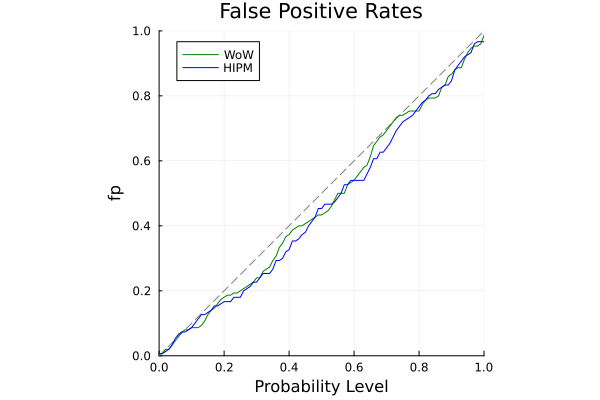
\includegraphics[width = \linewidth]{figures/ch5/normal_normal/falsepositive_rates_normal_normal_mu_1=1.0_n=35_m=10_s=150_permutations=80_samemeasures.png}
%     \end{subfigure}
%     \begin{subfigure}{0.32\textwidth}
%         \centering
%         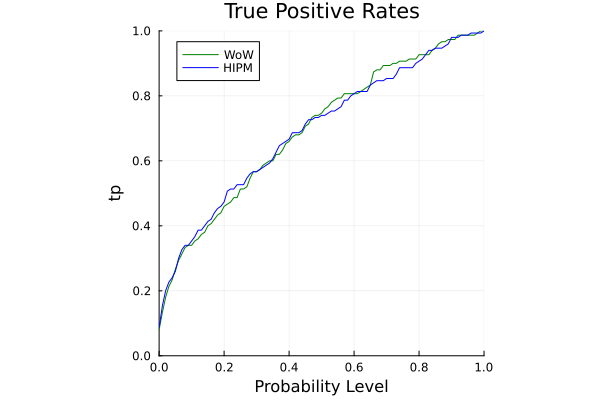
\includegraphics[width = \linewidth]{figures/ch5/normal_normal/truepositive_rates_normal_normal_mu_1=1.0_mu_2=1.5_n=35_m=10_s=150_permutations=80_diffmeasures.png}
%     \end{subfigure}
%     \begin{subfigure}{0.32\textwidth}
%         \centering
%         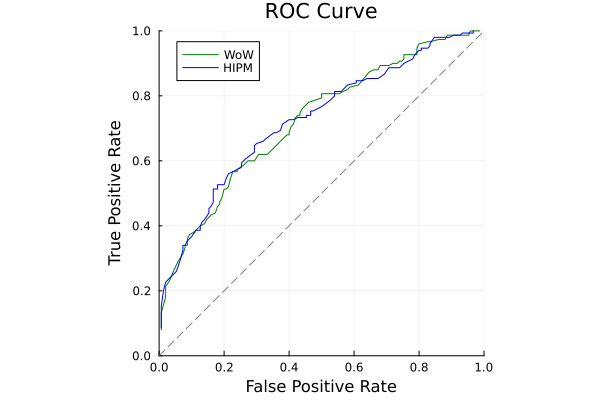
\includegraphics[width = \linewidth]{figures/ch5/normal_normal/ROC_normal_normal_mu_1=1.0_mu_2=1.5_n=35_m=10_s=150_permutations=80.png}
%     \end{subfigure}

%     \begin{subfigure}{0.32\textwidth}
%         \centering
%         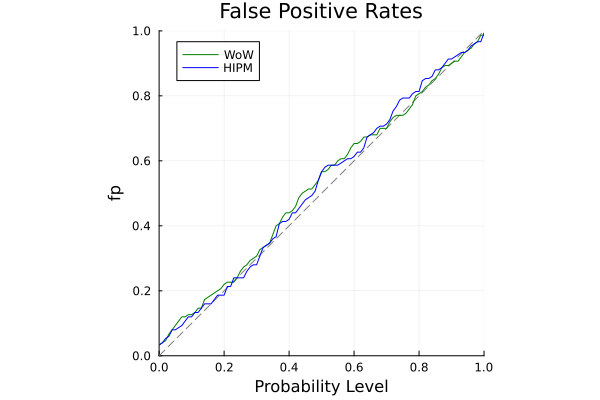
\includegraphics[width = \linewidth]{figures/ch5/normal_normal/falsepositive_rates_normal_normal_mu_1=1.0_n=70_m=15_s=150_permutations=80_samemeasures.png}
%     \end{subfigure}
%     \begin{subfigure}{0.32\textwidth}
%         \centering
%         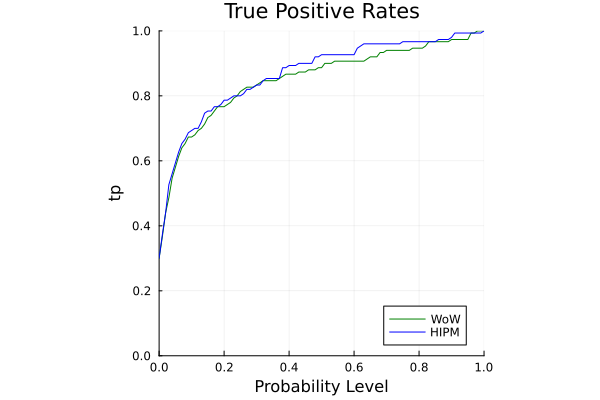
\includegraphics[width = \linewidth]{figures/ch5/normal_normal/truepositive_rates_normal_normal_mu_1=1.0_mu_2=1.5_n=70_m=15_s=150_permutations=80_diffmeasures.png}
%     \end{subfigure}
%     \begin{subfigure}{0.32\textwidth}
%         \centering
%         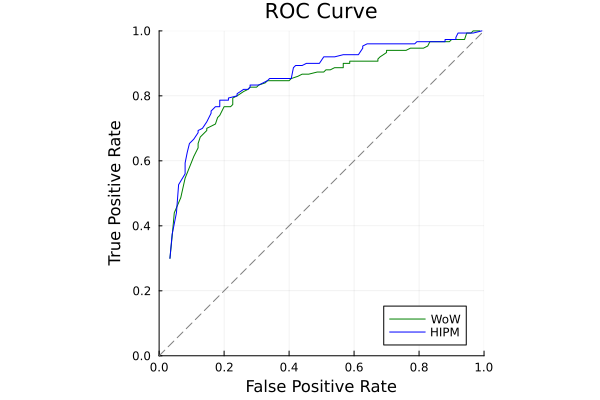
\includegraphics[width = \linewidth]{figures/ch5/normal_normal/ROC_normal_normal_mu_1=1.0_mu_2=1.5_n=70_m=15_s=150_permutations=80.png}
%     \end{subfigure}
%     \caption{}
%     \label{fig:normal_normal}
% \end{figure}

% As we see from the plot, for both of the distance functions, the Type I error is well controlled. Also, type II error is becoming low as we increase $n$ and $m$. In addition, the ROC curve is much better for both distance functions than the random guessing.

% What is not expected from the simulations is that we also control Type I error for the Wasserstein over Wasserstein. In theory, we could not show that under the null hypothesis, the test statistic has the same convergence properties as that with HIPM; however, in practice, it performs well. 

% In Figure~\ref {fig:DP_DP}, we are working with the same Dirichlet processes as the ones we used for Figure~\ref{fig:radem_threshold_plots}.

% Here, on the first row $n = 70, m = 7$, and on the second row $n = 120, m = 70.$ 

% \begin{figure}[H]
%     \centering
%     \begin{subfigure}{0.32\textwidth}
%         \centering
%         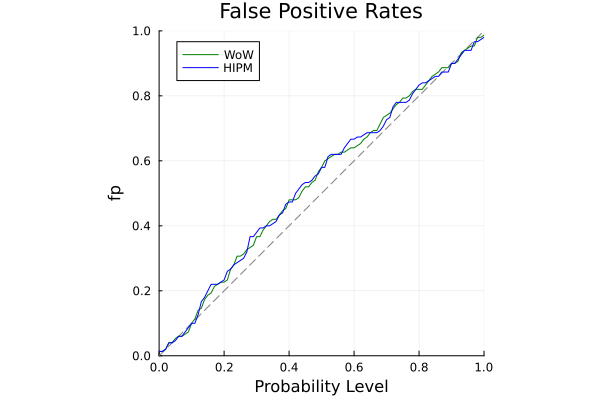
\includegraphics[width = \linewidth]{figures/ch5/dirichlet/falsepositive_rates_dirichlet_diffalpha_n=70_m=7_s=150_permutations=80_samemeasures.png}
%     \end{subfigure}
%     \begin{subfigure}{0.32\textwidth}
%         \centering
%         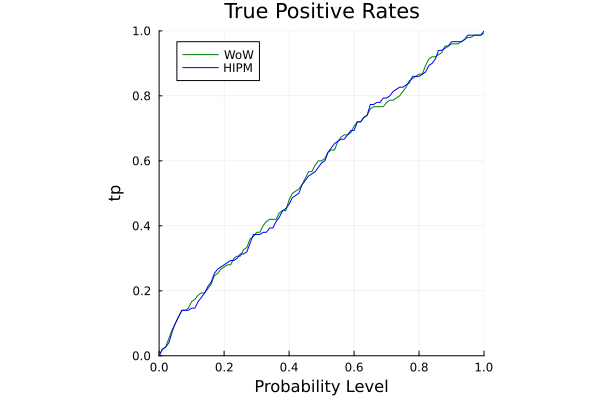
\includegraphics[width = \linewidth]{figures/ch5/dirichlet/truepositive_rates_dirichlet_diffalpha_n=70_m=7_s=150_permutations=80_diffmeasures.png}
%     \end{subfigure}
%     \begin{subfigure}{0.32\textwidth}
%         \centering
%         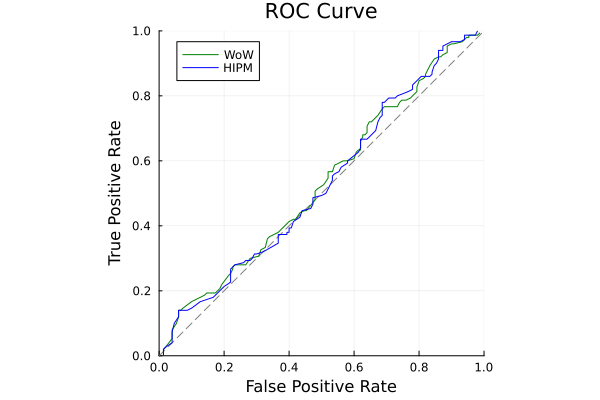
\includegraphics[width = \linewidth]{figures/ch5/dirichlet/ROC_dirichlet_diffalpha_alpha_1=1.0_alpha_2=1.5_n=70_m=7_s=150_permutations=80.png}
%     \end{subfigure}

%     \begin{subfigure}{0.32\textwidth}
%         \centering
%         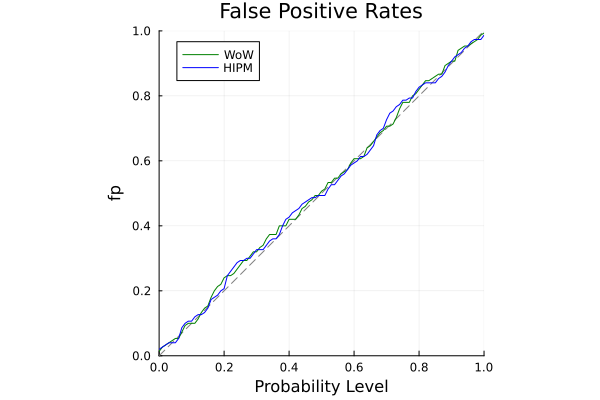
\includegraphics[width = \linewidth]{figures/ch5/dirichlet/falsepositive_rates_dirichlet_diffalpha_n=120_m=70_s=150_permutations=80_samemeasures.png}
%     \end{subfigure}
%     \begin{subfigure}{0.32\textwidth}
%         \centering
%         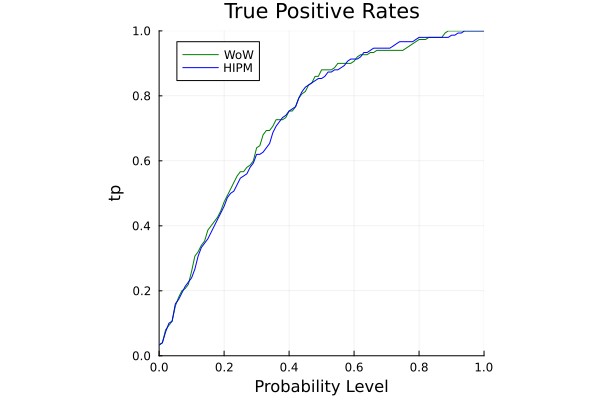
\includegraphics[width = \linewidth]{figures/ch5/dirichlet/truepositive_rates_dirichlet_diffalpha_n=120_m=70_s=150_permutations=80_diffmeasures.png}
%     \end{subfigure}
%     \begin{subfigure}{0.32\textwidth}
%         \centering
%         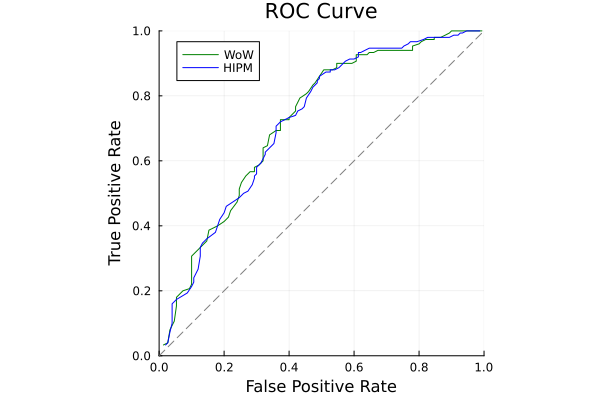
\includegraphics[width = \linewidth]{figures/ch5/dirichlet/ROC_dirichlet_diffalpha_alpha_1=1.0_alpha_2=1.5_n=120_m=70_s=150_permutations=80.png}
%     \end{subfigure}
%     \caption{}
%     \label{fig:DP_DP}
% \end{figure}


% As we see from the plot, for both of the distance functions, the Type I error is well controlled. Also, type II error is becoming low as we increase $n$ and $m$. In addition, the ROC curve is much better for both distance functions than the random guessing.

% What is not expected from the simulations is that we also control Type I error for the Wasserstein over Wasserstein. In theory, we could not show that under the null hypothesis, the test statistic has the same convergence properties as that with HIPM; however, in practice, it performs well. 

% In Figure~\ref {fig:DP_DP}, we are working with the same Dirichlet processes as the ones we used for Figure~\ref{fig:radem_threshold_plots}.
% Similarly to the Figure~\ref{fig:normal_normal}, in Figure~\ref{fig:DP_DP}, we also see that the Type I error is well controlled. Here, the true positive rate is improving slowly as we increase $n$ and $m$ but this is because the $\alpha$'s we chose for random probability measures are very close to each other. 







% For a given probability level $\theta,$ if the frequency of those samples exceeding the observed distance is smaller than $\theta,$ this means that the observed distance is larger than the empirical $(1-\theta)$-quantile from those samples. Even though in practice we consider a finite number of permutations, to study the theoretical properties of this approach we define the permutation threshold at probability level $\theta$ as the $(1 - \theta)$-quantile of the random variable 
% $$ 
% \widetilde{T}_{n,m} = \sqrt{\frac{n}{2}} \, d(\widetilde{Q}^1_{n,m}, \widetilde{Q}^2_{n,m}), 
% $$
% where the only source of randomness is the permutation, and $\{ \widehat{P}^1_{1,m},\ldots,\widehat{P}^1_{n,m},\widehat{P}^2_{1,m},...\widehat{P}^2_{n,m} \}$ are fixed. Note that here we have the factor $\sqrt{\frac{n}{2}}.$ Note that in this case, the test statistic is 
% \[
% T_{n,m} = \frac{n}{2}\dlip\left( \widehat{Q}^1_{n,m}, \widehat{Q}^2_{n,m} \right).
% \]
% Comparing empirical quantile from permuted samples to the observed distance $d(\widehat{Q}^1_{n,m}, Q^2_{n,m
% })$ is equivalent to comparing their associated scaled versions to each other. This scaling factor is needed to study the asymptotic distribution of random variables $T_{n,m}$ and $\widetilde{T}_{n,m}.$

% The testing scheme has the following structure: after observing hierarchical samples $\mathbf{X}\sim Q^1$ and $\mathbf{Y}\sim Q^2,$ we obtain the samples $\widetilde{T}^1_{n,m}, ..., \widetilde{T}^S_{n,m}$ from the permutation approach, and reject the null hypothesis if 
% \[
% T_{n,m} > \widehat{c}(n,m,\theta),
% \]
% where $\widehat{c}(n,m,\theta)$ is the empirical quantile of the random variable $\widehat{T}_{n,m}$ computed from the samples $\widetilde{T}^1_{n,m}, ..., \widetilde{T}^S_{n,m}.$ 

% Note that it is equivalent to reject $H_0$ if 
% $$
% \frac{1}{S}\sum_{i = 1}^S \mathbf{1}\!\left(T_{n,m} < \widetilde{T}^i_{n,m}\right) \leq \theta.
% $$
% To sum up, the algorithm has the following structure: 

% \begin{algorithm}
% \caption{Permutation Test: Reject/Do Not Reject $H_0$, $ d \in \{\dlip,\WW\}$ }
% \label{algorithm:permutation_approach}
% \begin{algorithmic}[1]
% \Require Hierarchical samples $X, \mathbf{Y}$; significance level $\theta$; number of permutations $n_{\mathrm{perm}}$
% \Ensure Decision: $1=$Reject $H_0$, $0=$Do not reject $H_0$

% \State $d_{\mathrm{obs}} \gets d(X, \mathbf{Y})$ \hfill \Comment{Compute observed distance}
% \State $Pooled\_sample \gets \mathrm{concat}(X, \mathbf{Y})$ \hfill \Comment{Pool both samples}
% \State $n \gets \text{number of rows in } X$
% \State $permuted\_distances \gets [\ ]$ \hfill \Comment{Initialize storage for permuted distances}

% \For{$b = 1$ to $n_{\mathrm{perm}}$}
%   \State $R \gets$ random permutation of $\{1, \dots, 2n\}$
%   \State $X' \gets Pooled\_sample[{R(1:n)}]$ \hfill \Comment{choose first $n$ random rows from pooled samples}
%   \State $\mathbf{Y}' \gets Pooled\_sample[{R(n+1:2n)}]$ \hfill \Comment{choose second $n$ random rows from pooled samples}
%   \State append $d(X', \mathbf{Y}')$ to $permuted\_distances$
% \EndFor

% \State $t_{\theta} \gets \operatorname{Quantile}(permuted\_distances,\,1 - \theta)$ \hfill \Comment{Compute threshold}
% \State \Return $\mathbbm{1}\{\,d_{\mathrm{obs}} > t_{\theta}\,\}$ \hfill \Comment{Reject if observed distance exceeds threshold}
% \end{algorithmic}
% \end{algorithm}
% To study the theoretical properties of this testing scheme, we consider the behaviour of 
% $$
% \mathbb{P}\!\left(T_{n,m} > c(n,m,\theta)\right)
% $$
% under the null and alternative hypotheses, where $c(n,m,\theta)$ is the theoretical quantile of $\widetilde{T}_{n,m},$ defined as
% $$
% c(n,m,\theta) = \inf \left\{ t \in \R : \mathbb{P}\left(\widetilde{T}_{n,m} > t \right) \leq \theta \right\}.
% $$
% We will call $c(n,m,\theta)$ the permutation threshold.

% The theoretical guarantees are obtained by studying the asymptotic distributions of $T_{n,m}$ and $c(n,m,\theta).$ 